\subsection{Thời gian: Sắp xếp theo trình tự thời gian tuần hoàn}
Tominski và Schumann [416] sử dụng mã màu hai tông (two-tone) nâng cao của Saito và cộng sự [354] để trực quan hóa dữ liệu phụ chuỗi thời gian dọc theo hình xoắn ốc. Mỗi đơn vị khoảng thời gian được thể hiện bằng một đoạn duy nhất trên xoắn ốc. Mỗi phân đoạn được chia thành hai phần tô màu theo phương pháp tô màu hai tông. Ưu điểm của việc sử dụng phương pháp tô màu hai tông là nó giúp hiện thực hóa khái niệm tổng quan + chi tiết bằng một thiết kế trực quan. Hai màu được sử dụng trên mỗi đoạn xoắn ốc cho phép người dùng nhanh chóng nhận ra khoảng giá trị của đoạn đó (tổng quan). Nếu ta quan tâm tới một khoảng giá trị nhất định, tỷ lệ của hai màu sẽ giúp biểu thị giá trị dữ liệu cụ thể một cách chính xác (chi tiết). \textit{Xoắn ốc tương tác nâng cao} có thể được điều chỉnh tương tác theo nhiều cách khác nhau. Số lượng đơn vị giai đoạn thời gian, số chu kỳ và các tham số hình học bổ sung sẽ quyết định hình dạng của đường xoắn ốc. Việc biểu diễn dữ liệu chủ yếu được kiểm soát bởi các thang màu sắc đã sử dụng và các tham số như số lượng màu, hướng ánh xạ và chức năng ánh xạ (tuyến tính hay logarit). Việc điều hướng có thể được thực hiện tức thì thông qua việc điều chỉnh trực tiếp xoắn ốc.
\\ \\ 
Nội dung mục này và Hình (\ref{fig:f7.9}) minh họa một hình xoắn ốc nâng cao với mã màu hai tông. Mã giả dưới đây là một ví dụ minh họa cách vẽ một hình xoắn ốc đơn giản trong đó màu sắc và độ rộng của các thanh thể hiện độ lớn giá trị của dữ liệu tương ứng (so sánh hình ảnh ở giữa và bên phải trong Hình (\ref{fig:f7.1})). Các tham số đầu vào bao gồm dữ liệu (\textit{data[]}) - một mảng gồm n giá trị dữ liệu không âm với \textit{max} là giá trị lớn nhất. Tọa độ tâm của hình xoắn ốc được ký hiệu là \textit{cx} và \textit{cy}. Bán kính trong và bán kính ngoài của hình xoắn ốc được cho bởi các tham số \textit{inRad} và \textit{outRad}. Số lượng giá trị dữ liệu hiển thị trong một chu kỳ xoắn ốc đầy đủ, hay nói cách khác là số lượng đoạn thẳng trên mỗi chu kỳ được cho bởi tham số \textit{cyclLen}.
\begin{figure}[H] % places figure environment here   
    \centering % Centers Graphic
    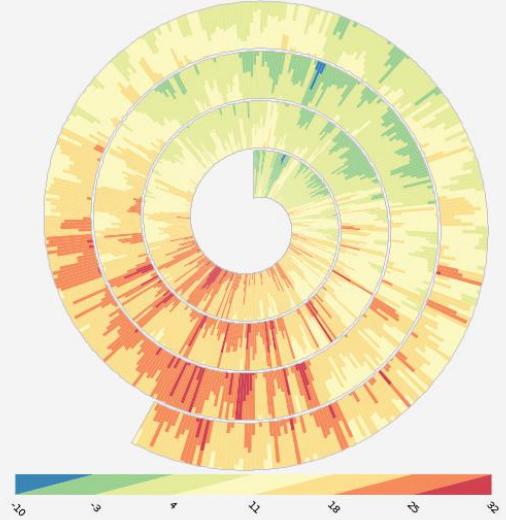
\includegraphics[width=0.8\textwidth]{assets/fig_7_9.png} 
    \caption{Xoắn ốc tương tác nâng cao [416]. Hình xoắn ốc biểu diễn dữ liệu thời tiết trong 3 năm 6 tháng. Mỗi chu kỳ thể hiện 365 giá trị nhiệt độ trung bình hàng ngày ở thành phố Rostock. Ta có thể thấy mùa đông những năm gần đây (chu kỳ ngoài cùng) có khí hậu ôn hòa hơn so với các mùa đông trước. (Nguồn: Hình vẽ được thực hiện bằng công cụ biểu diễn xoắn ốc tương tác nâng cao.)} % Creates caption underneath graph
    \label{fig:f7.9}
\end{figure}